\chapter*{Cinematica}

    \section*{Moto rettilineo uniforme}

        \subsection*{Velocità} 
            \begin{equation*}
                v_x = k \; [m/s]
            \end{equation*}

        \subsection*{Velocità media} 
            \begin{equation*}
                v_m = \frac{\Delta x}{\Delta t} = \frac{x_f - x_i}{t_f - t_i}
            \end{equation*}

        \subsection*{Velocità istantanea}
            \begin{equation*}
                v = \lim_{x \to 0}  \frac{\Delta x}{\Delta t} = \frac{dx}{dt}
            \end{equation*}

        \subsection*{Spostamento}
            \begin{equation*}
                x(t) = x_i + v_xt \; [m]
            \end{equation*}

    \section*{Moto uniformemente accelerato}

        \subsection*{Accelerazione media}
            \begin{equation*}
                a_m = \frac{\Delta v}{\Delta t} = \frac{v_f - v_i}{t_f - t_i} 
                \, [m/s^2]
            \end{equation*}

        \subsection*{Accelerazione istantanea}
            \begin{equation*}
                a = \frac{dv}{dt} = \frac{d^2x}{dt^2}
            \end{equation*}

        \subsection*{Spostamento}
            \begin{equation*}
                x(t) = x_i + v_it + \frac{1}{2}at^2 \; [m]
            \end{equation*}

        \subsection*{Velocità finale}
            \begin{equation*}
                v_f(t) = v_{i} + at
            \end{equation*}
    
        \subsection*{Caso particolare: tempo non dipendente dalla massa}
            \begin{equation*}
                t_c=\sqrt{\frac{2h}{g}} \; [s]
            \end{equation*}

    \section*{Moto di un proiettile} 
        \begin{itemize}
            \item \textbf{Asse X}: moto rettilineo uniforme.
            \item \textbf{Asse Y}: moto rettilineo uniformemente accelerato.
        \end{itemize}
        \subsection*{Equazioni del moto}
        (Per assi cartesiani)
        \begin{align}
            \textsf{Moto} &: \begin{cases}
                    x(t) &= x_0 + v_{0x}t \\
                    y(t) &= y_0 + v_{0y}t + \frac{1}{2}at^2
                \end{cases} \\
                \textsf{Velocità} &: v_{f} = v_{0} + at
        \end{align}

    \section*{Moto circolare uniforme}

        \subsection*{Velocità tangenziale} 
            \begin{equation*}
                v = \frac{2\pi r}{T} \; [m/s]
            \end{equation*}

        \subsection*{Accelerazione centripeta}
            \begin{equation*}
                a_c = \frac{v^2}{r} \; [m/s^2]
            \end{equation*}

        \subsection*{Periodo}
            \begin{equation*}
                T = \frac{2\pi r}{v} \; \Bigg[N = \frac{Kg \cdot m}{s^2} \Bigg]
            \end{equation*}
        
        \subsection*{Velocità angolare}
            \begin{equation*}
                \omega = \frac{2\pi}{T} \, \Bigg[\frac{rad}{s} \Bigg]
            \end{equation*}
        Espressa in radianti al secondo.
    
    \section*{Moto Armonico}

        \subsection*{Legge oraria (equazione del moto)} 
        \begin{equation*}
            \Theta = \Theta_0 + \omega t = 
            \begin{cases}
                x(t)=R\cos{\Theta(t)} \\
                y(t)=R\sin{\Theta(t)}
            \end{cases} 
            = 
            \begin{cases}
                x(t)=R\cos{(\Theta_o+\omega t)} \\
                y(t)=R\sin{(\Theta_o+\omega t)}
            \end{cases}
        \end{equation*}

        \subsection*{Velocità tangenziale}
            \begin{equation*}
                v = \frac{2\pi r}{T} = 
                \begin{cases}
                    v_x=-R\omega\sin{(\Theta_o+\omega t)} \\
                    v_y=R\omega\cos{(\Theta_o+\omega t)}
                \end{cases}
            \end{equation*}

        \subsection*{Accelerazione centripeta} 
            \begin{equation*}
                a_c = \frac{v^2}{r}=
                \begin{cases}
                    a_x=-R\omega^2\cos{(\Theta_o+\omega t)} \\
                    a_Y=-R\omega^2\sin{(\Theta_o+\omega t)}\end{cases}
            \end{equation*}
        
    \section*{Moto circolare uniformemente accelerato}

        \subsection*{Legge oraria (equazione del moto)}
            \begin{equation*}
                \begin{cases} 
                    \Theta = \Theta_0 + \omega_0t + \frac{1}{2}\alpha t^2 \\ 
                    \omega = \omega_0+\alpha t
                \end{cases}
            \end{equation*}

        \subsection*{Tabelle di riepilogo} Di seguito sono riportate due 
        tabelle contententi un riepilogo delle formule (comprese le formule 
        inverse) sia del Moto circolare uniforme \ref{fig:MCU} che del Moto 
        circolare uniformemente accelerato \ref{fig:MCUA}.

        \begin{figure}[H]
            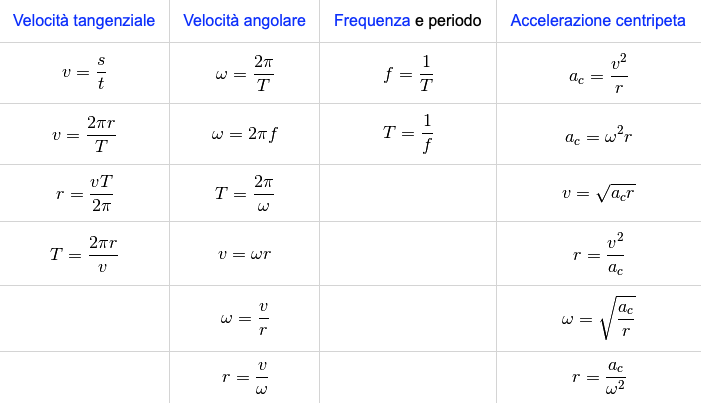
\includegraphics[width=0.9\linewidth]
            {formulario/img/Formulario_MCU.png}
            \caption{Formule del Moto circolare uniforme}
            \label{fig:MCU}
        \end{figure}

        \begin{figure}[H]
            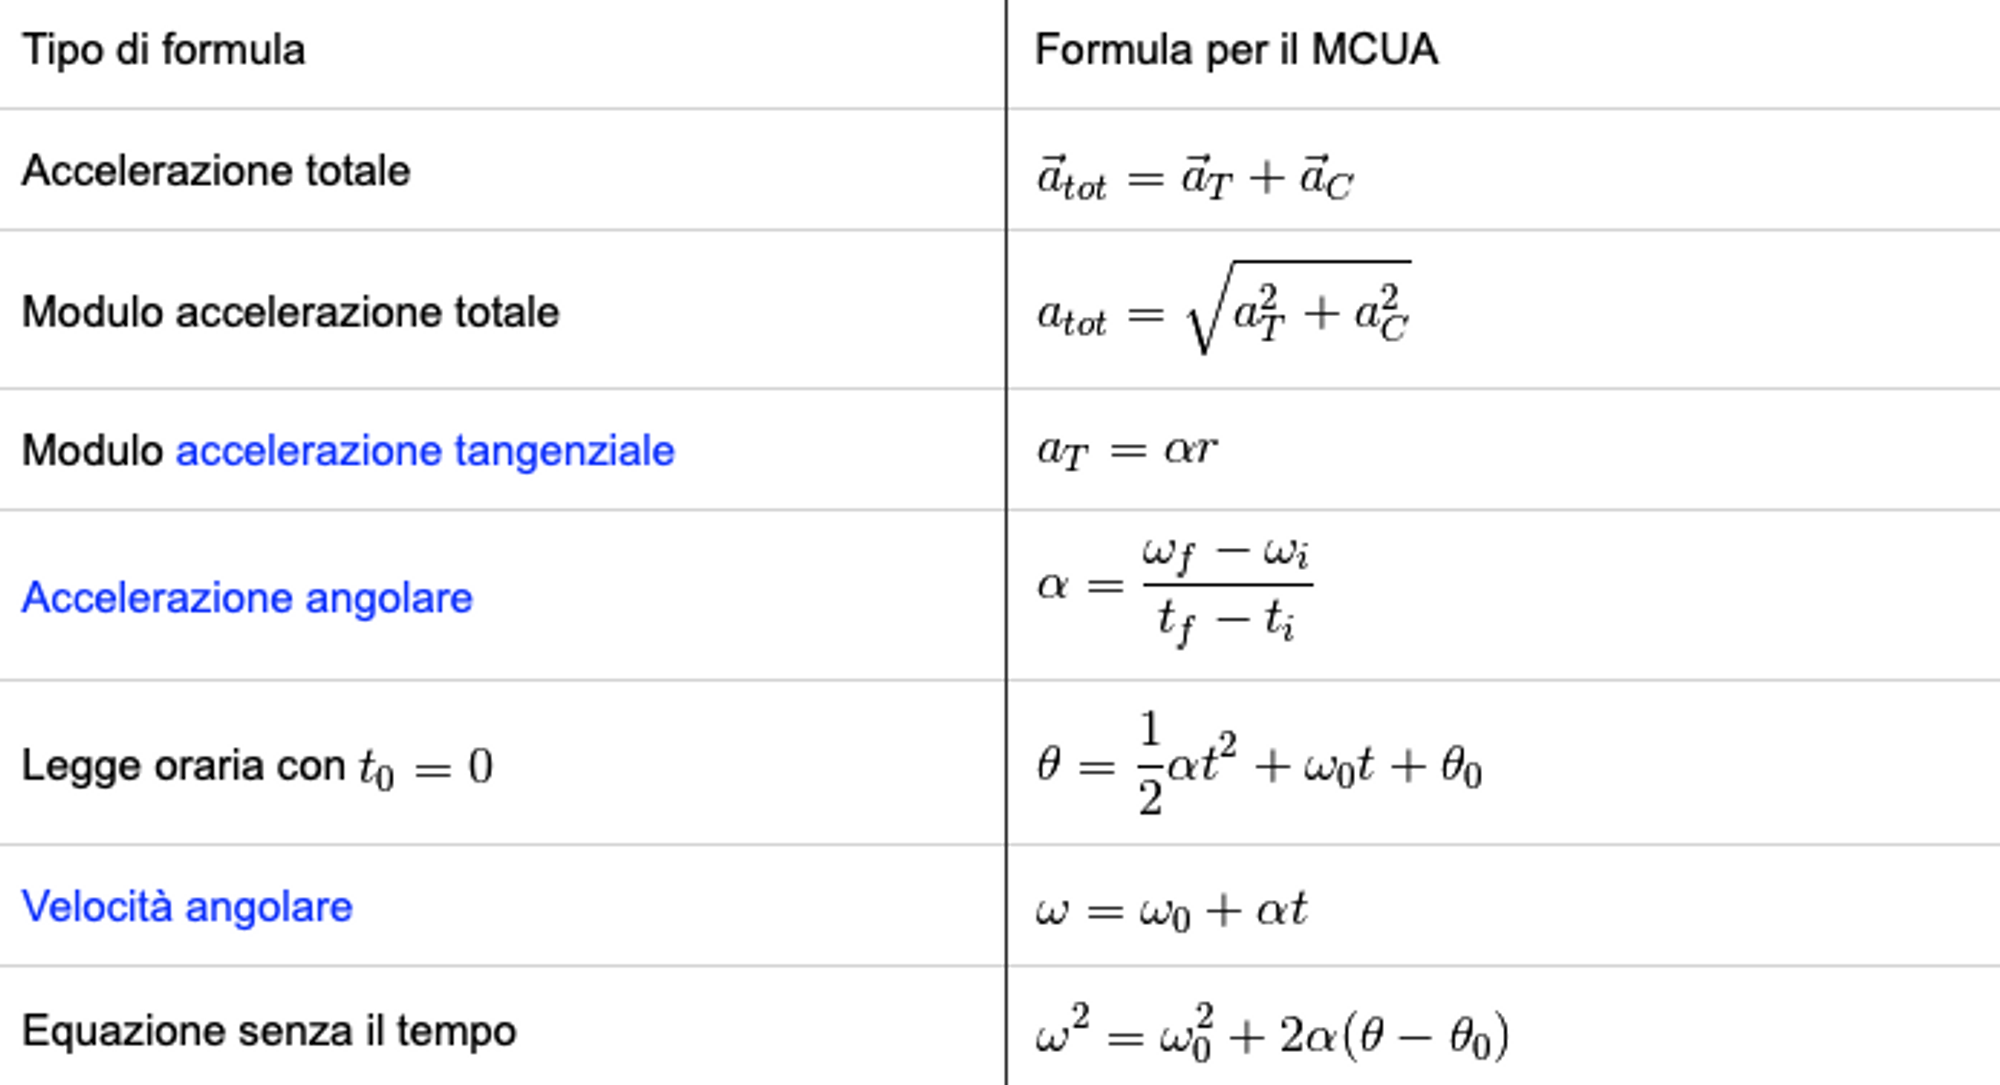
\includegraphics[width=0.9\linewidth]
            {formulario/img/Formulario_MCUA.png}
            \caption{Formule del Moto circolare uniformemente accelerato}
            \label{fig:MCUA}
        \end{figure}

        